\subsection{Tratamiento de datos faltantes}

\textbf{Descripción}: En la práctica, es común encontrarse y tener que trabajar con datasets que
contienen datos nulos o incompletos. Existen distintos métodos para tratar con ellos, en esta sección
se exploraron dos. Los cuales tratan de rellenar los datos faltantes con el valor modal del
atributo, y se diferencian en que uno toma en cuenta el valor de la clase para el individuo o registro
analizado, mientras que el otro no tiene en cuenta el valor de la clase.


\textbf{Metodología utilizada}:
Para el tratamiento de datos faltantes se indujo valores nulos al 80\% del dataset en los atributos con mayor GainRatio,
se preservó el 20\% de los datos para validación. A continuación se detallan las características de los atributos contemplados:

\definecolor{lightgray}{gray}{0.9}
\begin{table}[H]
\begin{center}
\caption{Atributos con mayor GainRatio}
\rowcolors{1}{}{lightgray}
\begin{tabular}{|>{\centering\arraybackslash}m{3cm}|>{\centering\arraybackslash}m{3cm}|}
\hline
  \rowcolor{blue!55} 
   \multicolumn{1}{|c|}{Atributo} &\multicolumn{1}{c|}{GainRatio} \\ \hline
    inst\_acreditada   &0.0436292021  \\ \hline
    estu\_metodo\_prgm &0.0295357038  \\ \hline
    \end{tabular}
\label{Gain Ratio}
\end{center}
\end{table}

El porcentaje de imputación de datos faltantes fue variando de 0 a 0.85 con incrementos de 0.025 generando
36 datasets con datos faltantes. 
En cada generación de datos faltantes, se relleno con la  moda los datos nulos del atributo inst\_acreditada  y con la modaclase para 
los valores nulos del atributo estu\_metodo\_prgm. Después se construyeron modelos con las estrategias
de relleno de datos faltantes anteriormente descritas variando el CF (Confidence Factor) de 0 a 0.5 y 
finalmente se evaluaron los mismos con el set de validación.

\textbf{Resultados esperados}: La performance sobre el set de validación no debería verse
sensiblemente afectada, al menos al introducir proporciones bajas o medias de datos faltantes, 
dada la robustez del algoritmo J48 para lidiar con esta problemática. 

Con respecto al tamaño del árbol, es de esperar que el mismo aumente
a medida que aumenta la función de poda y no por el porcentaje inducido de datos faltantes. 

\textbf{Análisis de los resultados}: En la figura~\ref{fig:missing}a,
se observa un patrón de comportamiento en las curvas de entrenamiento y validación para la accuracy,
dicho patron es similar a las curvas generadas en las corridas donde no se imputaron datos faltantes,
esto nos dice que el algoritmo J48 presenta resistencia y robustez a datos faltantes, 
ya que la performance se ve afectada más por la función de poda que por la imputación de datos faltantes.

En la figura~\ref{fig:missing}b, 
se observa claramente que el tamaño del árbol  incrementa debido al aumento de la función de poda 
(confidence factor), respecto al porcentaje de datos faltantes no se mira que este afecte en el tamaño del arbol.

En la figura~\ref{fig:missing}c, se observa un comportamiento similar
para los diferentes porcentajes de datos faltantes imputados,  la presición se comporta de igual forma manteniendo
la variación debido a la función de poda independientemente del porcentaje de datos faltantes.

Los anteriores supuestos los podemos confirmar claramente en la figura~\ref{fig:missing}d,
donde se puede mirar que a valores bajos CF hay un alto performance en el set de datos de validación, y a
medida que aumenta el valor de CF (eje x), también aumenta el valor de la performance del set de entrenamiento (tamaño
de la burbuja) así como baja la performance del set de testing (color de la burbuja) por este motivo el arbol se sobre ajusta
al conjunto de entrenamiento. 
Esta lectura es posible realizarla según el porcentaje de datos faltantes (de 0 a 0,85, en el eje Y; Cada serie de burbujas horizontales
corresponden al mismo experimento).

\textbf{Conclusión:} Los resultados se presentaron, en mayor o menor medida, en línea con lo esperado. La performance no 
se vio sensiblemente deteriorada al igual que el tamaño del árbol, aliniandose a los resultados esperados. 
Por tanto  el algoritmo de árboles J48 es robusto a datos faltantes,
ya que el rendimiento y  tamaño del árbol observados en los gráficos  se ven afectados por la función de poda y no por la
variación de datos faltantes.


\begin{figure*}
  \centering
  \subfigure[Accuracy vs CF]{\label{b1} 
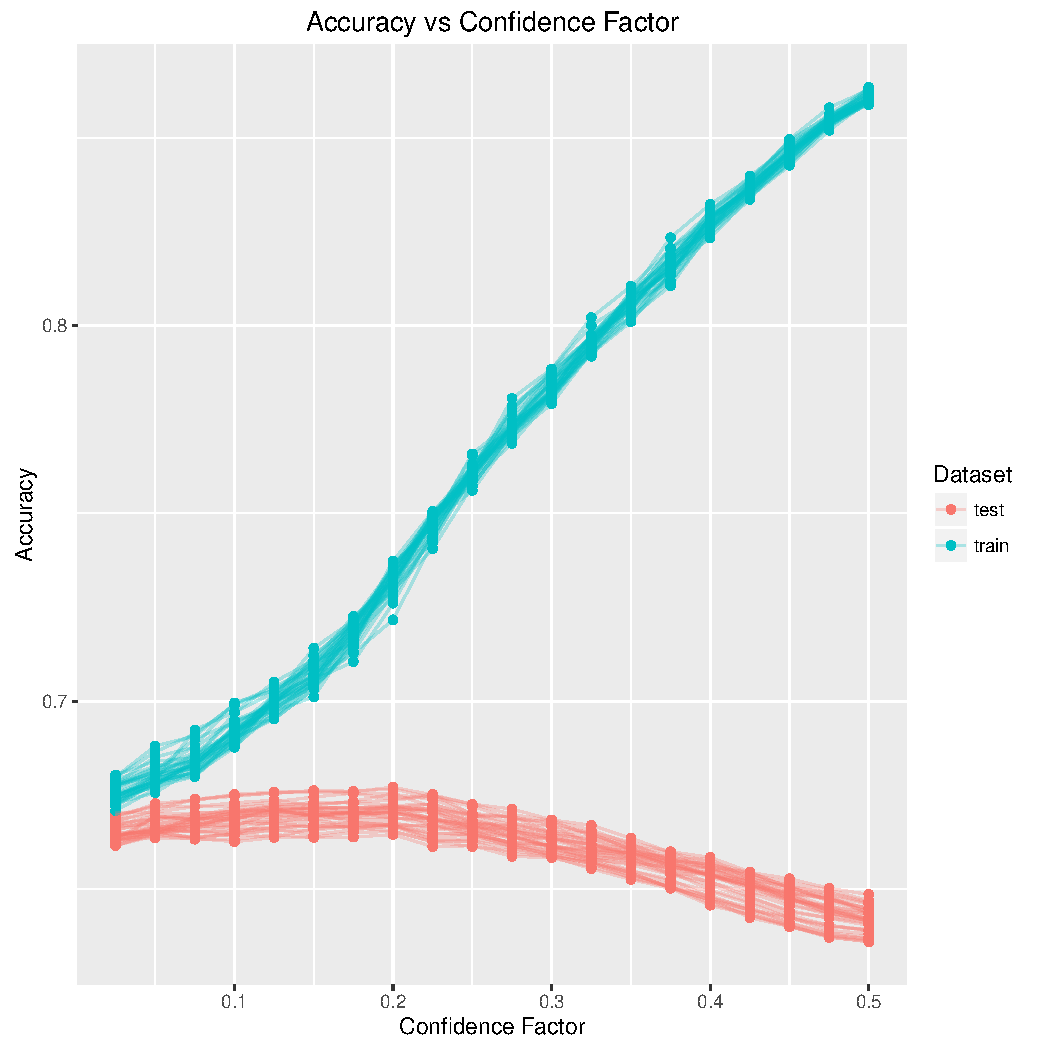
\includegraphics[width = 7cm]{4a.pdf}}
  \subfigure[Leaves vs missing percentage]{\label{b2} 
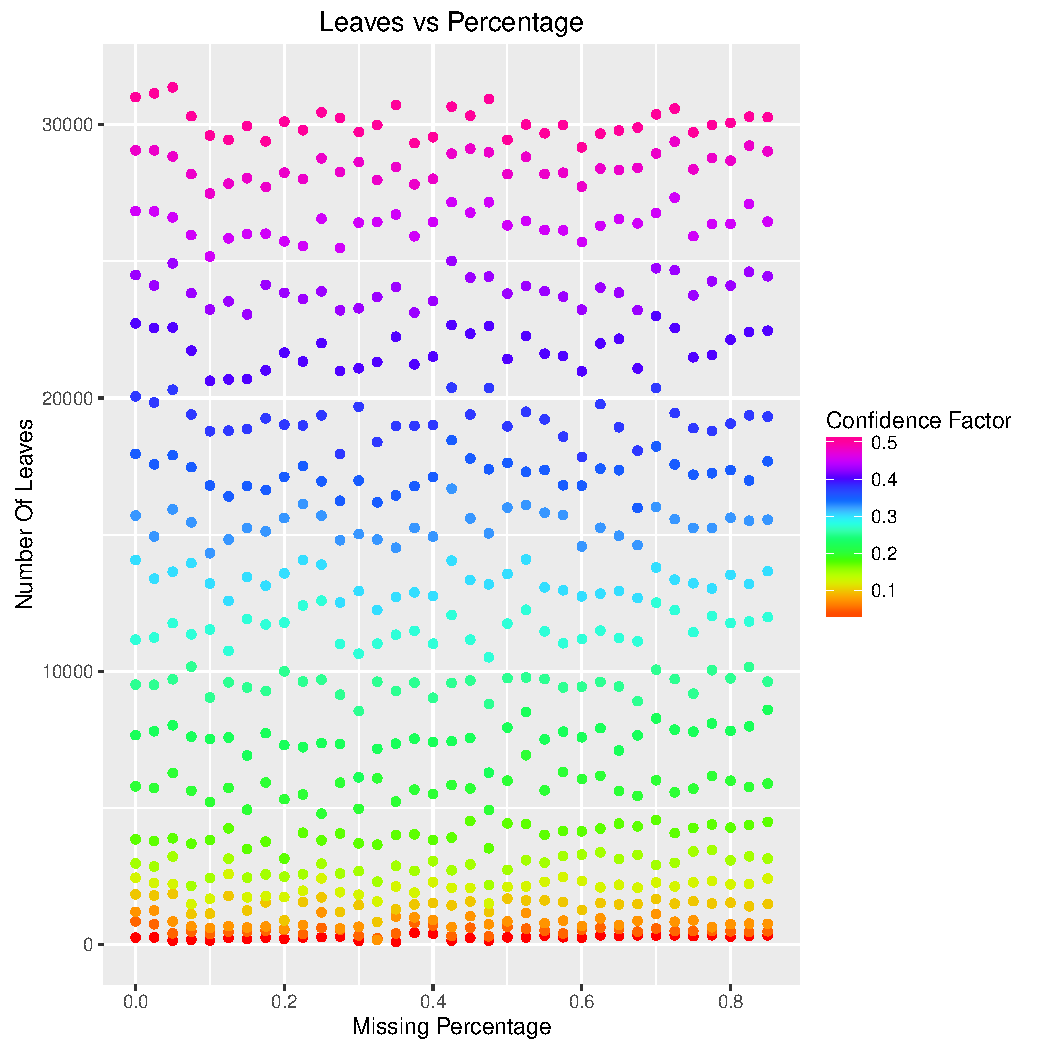
\includegraphics[width = 7cm]{4b.pdf}}
  \subfigure[Accuracy vs missing percentage]{\label{b3}
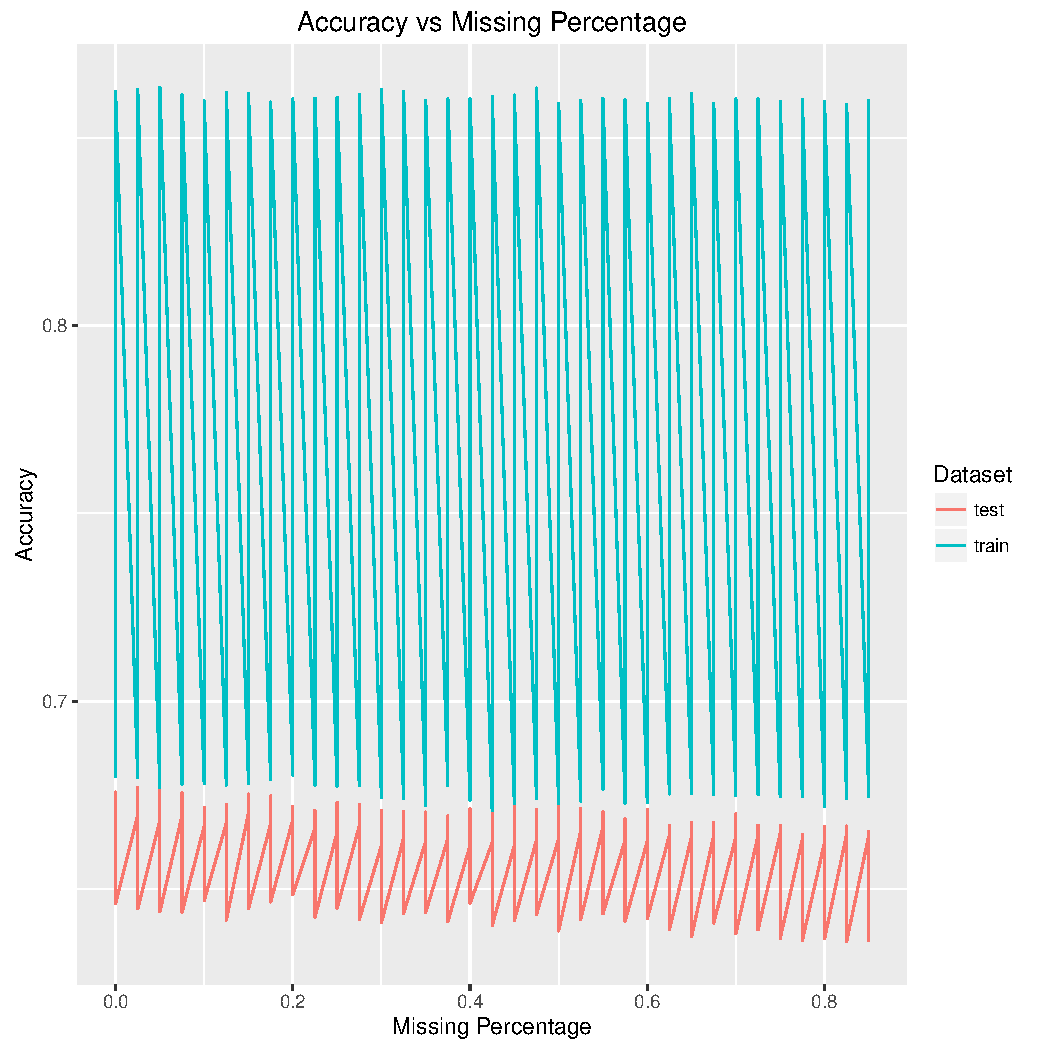
\includegraphics[width = 7cm]{4c.pdf}}
    \subfigure[Missing percentage vs CF]{\label{b4}
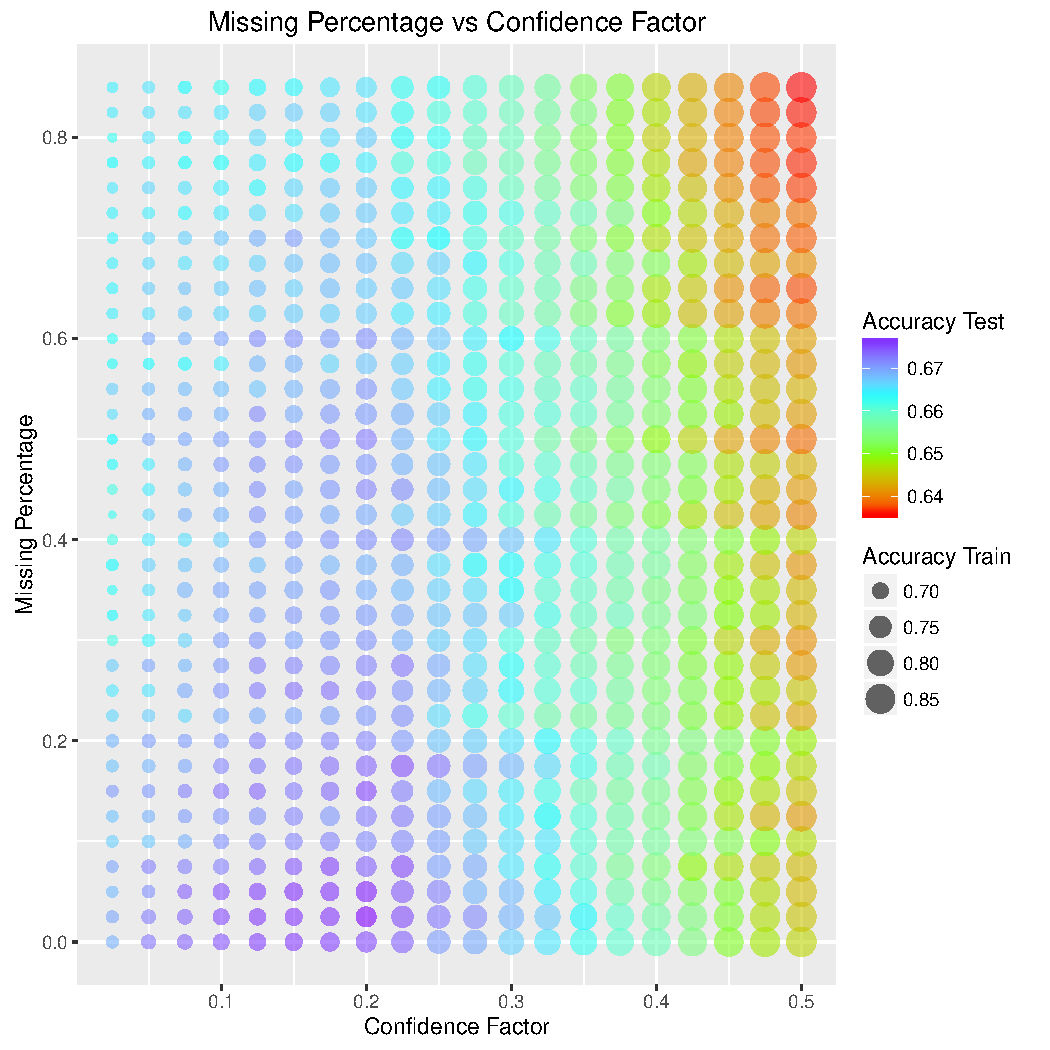
\includegraphics[width = 7cm]{4d.pdf}}
  \caption{Missing data}
  \label{fig:missing}
\end{figure*}
